\begin{figure}[H]
    \centering
    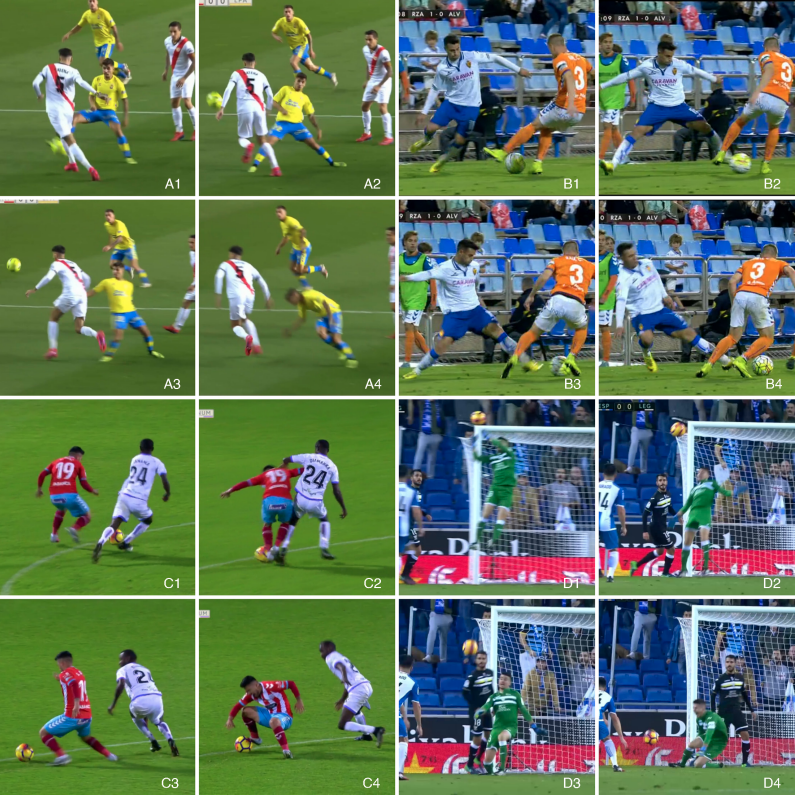
\includegraphics[width=0.85\textwidth]{images/patrones_movimiento_futbol.png}
    \caption{Patrones situacionales principales asociados a lesiones del ligamento cruzado
    anterior en fútbol profesional.
    (A) Presión (\textit{pressing}) (jugador con camiseta amarilla, lesión del LCA derecho):
    aproximación/presión sobre el oponente (A1), contacto inicial del pie derecho con el suelo
    (A2), instante estimado de lesión del LCA derecho (A3), pérdida del equilibrio (A4).
    (B) Quite o entrada defensiva (\textit{tackling}) (jugador con camiseta blanca, lesión del
    LCA derecho): aproximación/presión sobre el oponente (B1), contacto inicial del pie derecho
    con el suelo e intento de quite (B2), instante estimado de lesión del LCA derecho (B3),
    pérdida del equilibrio (B4).
    (C) Ser tackleado o recibir la entrada del rival (\textit{being tackled}) (jugador con
    camiseta roja, lesión del LCA derecho): presión ejercida por el jugador oponente (C1),
    perturbación mecánica/contacto del jugador defensor (C2), instante estimado de lesión del
    LCA derecho (C3), pérdida del equilibrio (C4).
    (D) Aterrizaje tras un salto (\textit{landing from a jump}) (arquero, uniforme verde, lesión
    del LCA derecho): salto (D1), contacto inicial de ambos pies con el suelo (D2), instante
    estimado de lesión del LCA derecho (D3), pérdida del equilibrio (D4).
    LCA: ligamento cruzado anterior. Fuente: adaptado de \textcite{BuckthorpeEtAl2024ACL}.}
    \label{fig:patrones_movimiento_futbol}
\end{figure}
